Before we look at the evolution of the wave field over tens of kilometers and hours time scale, it is 
worth looking at consequences of the shape of the wave spectrum 
on fluctuations in wave properties at the scale of few minutes and kilometers.
Indeed, the fact that waves are random introduces small scale variations. Most early work 
was focused on defining the statistics of series of high waves \citep{Arhan&Ezraty1978,Masson&Chandler1993}, which can be useful for example when catching 
waves on a surfboard, avoid the high waves when navigating a landing craft through the surf zone, or landing a helicopter on a ship. In this 
chapter we will start with another application which has become prominent as we are 
starting to look at smaller and smaller scale details in the wave field: estimating the expected 
fluctuations associated with groups \citep{DeCarlo&al.2023}, so that we may separate it from other effects, including 
refraction induced by currents and water depth, wave breaking, etc, which will be discussed in the 
following chapters. This investigation will also allow us to estimate lower bounds for uncertainties 
of wave measurements that will be defined from the time and space footprint of t{he measurements. The full uncertainty also contains instrument noise and measurement noise effects.

\section{Wave envelope, local amplitudes and their statistics}

Let $\zeta_c$ be the complex number such that $\zeta = \mathrm{Re}(\zeta_c)$ is the free surface, $\zeta_c$  is usally called the analytic signal. The envelope $\eta$ of the signal is defined by  $\eta = |\zeta_c|$, with an example shown in Fig. \ref{fig:groups1D}, using bottom pressure $p(z=-h)$ instead of surface elevation $\zeta$. 
%%%%%%%%%%%%%%%%%%%%%%%%%%%%%%%%%%%%%%%%%%%%%%%%%%%%%%%
\begin{figure}[htb]
\centerline{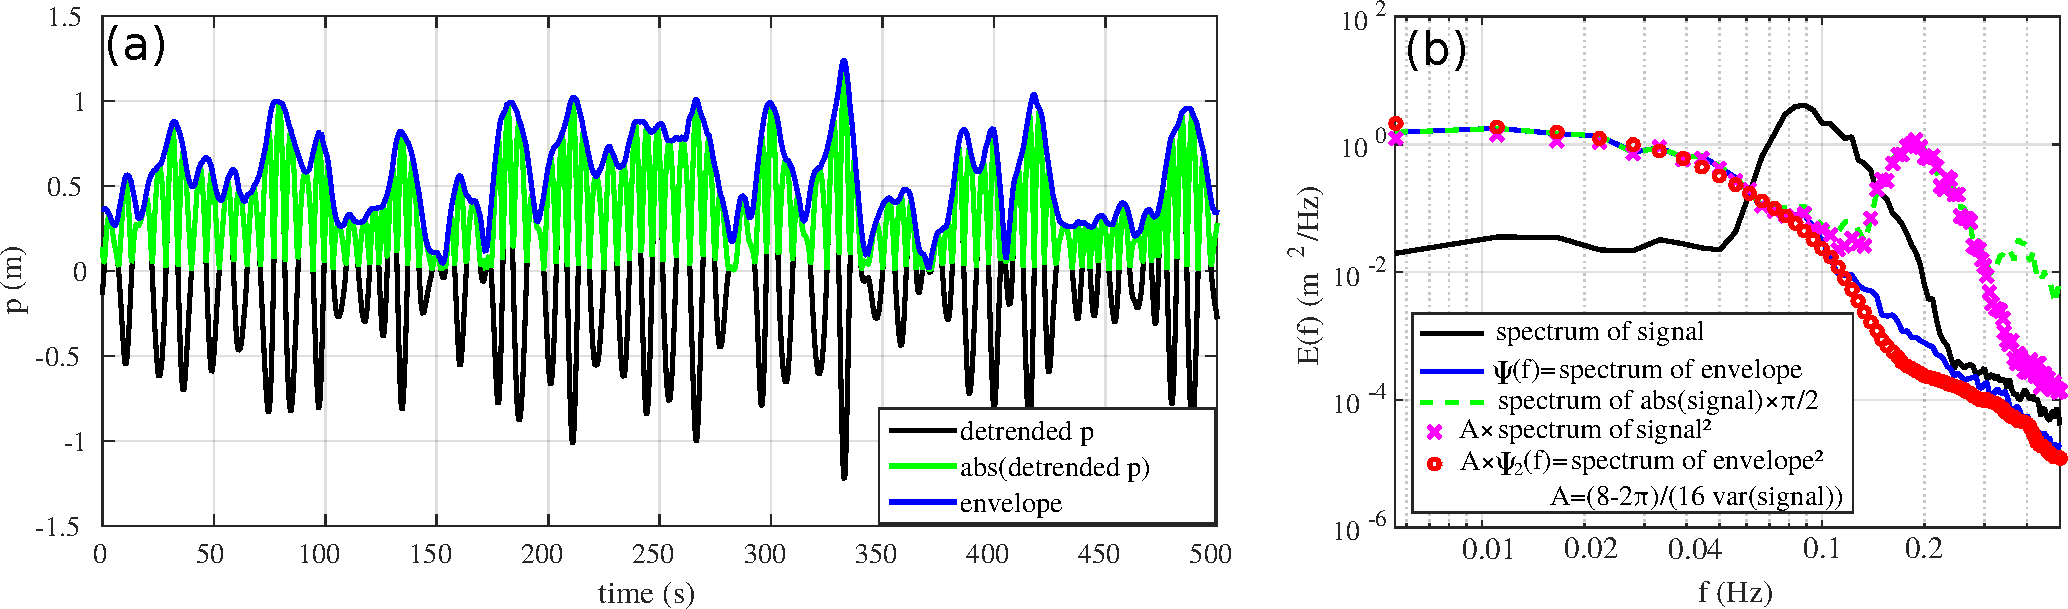
\includegraphics[width=\textwidth]{FIGS_CH_GROUPS/envelope_1D.pdf}}
%\vspace{3.64in}
  \caption{(a) time series of a signal, here the detrended ocean bottom pressure in Berthaume on January 31st 2004 (same data as in Figure 1.2), absolute value of the signal and signal envelope. (b) Spectra of the signal, the envelope, the rectified signal, and the approximate spectrum $\Psi_2$ obtained from a spectral convolution.}
\label{fig:groups1D}
\end{figure}
%%%%%%%%%%%%%%%%%%%%%%%%%%%%%%%%%%%%%%%%%%%%%%%%%%%%%%%
This defines a local amplitude of the signal that is continously defined everywhere. One interesting property of the envelope is that it does not contain the small scale crest-to-trough (positive to negative) variations of the original surface, so that its spectrum actually contains only longer components (larger periods in the case of time series). It is interesting to note that a similar operation is obtained by \emph{rectifying} the signal, i.e. taking its absolute value. This was particularly studied for electric signals by \cite{Rice1944} and the \emph{rectifier} in that case is a simple diode bridge. In the case of ocean waves, an important application is that of forces on moored ships, and you can think of the mooring line as a kind of rectifier, which will thus endure low-frequency forces. 

In fact it is easy to show that the signal and the rectified signal have the same mean squared value (i.e. the same integral of the spectrum including $f=0$), but they have very different spectra: the mean squared of the rectified signal is actually split half and half between sub-harmonics (very low frequencies) and super harmonics (higher than the peak frequency). Because the mean envelope squared is twice the mean rectified signal squared (if it is not obvious, think about it), then the envelope spectrum happens to be 4 times the spectrum of the rectified signal at low frequencies. 

The spectrum of the envelope turns out to be a pretty important quantity for many applications. Indeed, any non-linear effect will typically give the same kind of sub-harmonic and super-harmonic. In particular, any measurement device that is weakly non-linear will produce  spurious large scale fluctuations: this is the case of mooring lines for floating buoys, it is also the case of the KaRIN radar on board the SWOT satellite \citep{Peral&al.2015}. Separating the spurious signal from the real signal can involve the spectrum of the envelope. So you may be pleased to know that we can compute the spectrum of the envelope from the wave spectrum itself using the following approximation \citep{Tayfun&Lo1989}
\begin{equation}
    \Psi \simeq \frac{8 - 2\pi}{H_s^2}  \Psi_{2},
\label{eq:TayfunetLo}
\end{equation}
where $\Psi_2$ is the spectrum of the envelope squared and is obtain by convolving the wave spectrum with itself. This expression is valid for the surface elevation envelope. For any other quantity (orbital velocity, Stokes drift ...), just replace $H_s$ by 4 times the standard deviation of the quantity of interest. And before you complain that this is only an approximation, you may note that we have an exact equation for the spectrum of the envelope squared: if you enjoy the satifying beauty of exact equations please consider studying the fluctuations of the variances instead of the fluctuations of the amplitudes, and things will be very nice. 

We will now use this envelope spectrum to compute the expected fluctuations of wave measurements when estimated from a short record or a small area: here "short" or "small" is relative to the size of a few wave groups in time and space. The concept is the same when working with time series or two-dimensional maps, so we will treat both situations, starting with time series. 

\subsection{Time series}
From a time series $\zeta(t)$, the envelope can also be defined using the  Hilbert transform $\cal{H}(\zeta)$ of the time series, 
\begin{equation}
   \eta  = \left| \zeta + \cal{H}(\zeta) \right|.
   \label{eq:env_Hilbert}
\end{equation}
A practical calculation of the Hilbert transform is obtained using Fourier and inverse Fourier transforms. 


\subsubsection{Definition of a local wave height}
From the envelope $\eta$ we define the wave height $H_{r}$ as an average over a time segment of "radius" $\tau$
\begin{equation}
    H_{\tau}(t) = 4\sqrt{\frac{2}{\pi}} (\eta \otimes g_{\tau})(t)
   \label{eq:relation_Hs_eta}
\end{equation}
where $\otimes$ is the convolution operator and $g_{\tau}$ is a filtering kernel of radius $\tau$, more explicitly 
\begin{equation}
    H_{\tau}(t) = 4\sqrt{\frac{2}{\pi}} \int_{-\tau}^\tau \eta(t+u)   g_{\tau}(u) {\mathrm d}u
   \label{eq:relation_Hs_eta}
\end{equation}

Under the Gaussian approximation for the distribution of sea surface elevations this time average actually converges to the usual significant wave height $H_s$: the factor $\sqrt{{2}/{\pi}}$ is there simply to correct for the fact that the envelope is always above the rectified signal. 

Now, you may think of this filter $g_\tau$ as your "observation operator". I know, for time series it sounds a bit silly but there is always some kind of filter in the instrument, which can be the sensor itself or the effect of the structure that it is mounted on. If we consider the most simple case, our filter will be a box-car, taking the constant value $1/2\tau$ between $-\tau$ and $\tau$ and zero otherwise. What if we estimated the significant wave height as  $\widehat{H}_\tau$, with $\tau=64$~s? Some of these estimates would occur when a group of large waves is present, giving a large value, and others would give a lower value. In general, we may expect a variability, quantified by a variance $   \mathrm{var}(H_\tau)$. 

We can estimate this variance from the spectrum of the envelope $\Psi (f)$, by summing all the contributions from scales longer than $4 \tau$, i.e. frequencies lower than $1/(4 \tau)$, 
\begin{equation}
   \mathrm{var}(H_\tau) = \frac{32}{\pi} \int_0^{1/(4 \tau)} \Psi (f) {\mathrm d} f.
   \label{eq:relation_Hs_eta}
\end{equation}
We may also use the fact that the (single-sided) spectrum of the envelope squared  $\Psi_2(f)$ is the convolution of the spectrum of the single-sided
surface elevation spectrum $E(f)$ by itself,
\begin{equation}
    \Psi_{2}(f) = 8 \int_0^\infty E(u)E(u+f)\mathrm{d}u. 
\label{eq:psi2_1sided}
\end{equation}
 In practice people have rather studied the variations of $H_s$ and not that of $H_s^2$, 
 Although the details of the theory are more complex, the important result is that, for low frequencies, the spectrum of the envelope $\Psi(f)$ has the same shape as the spectrum of the envelope squared $\Psi_2(f)$ \citep{Rice1944}. More specifically, \cite{Tayfun&Lo1989} have showed that a good approximation for $\Psi$ is given by eq. (\ref{eq:TayfunetLo}). 

If $\tau$ is large enough, then the frequency $1/(2 \tau)$ will fall in the region where $\Psi(f) \simeq \Psi(f=0)$. For the case shown in Fig. \ref{fig:groups1D}, that cand be up to 0.02 or even 0.04~Hz. We can use this approximation to estimate the  variance of $\widehat{H}_\tau$ as
\begin{equation}
   \mathrm{var}(H_\tau)\simeq \frac{32}{\pi} \frac{\Psi (f=0)}{4 \tau} \simeq \frac{16(16 - 4 \pi) }{4 \pi \tau H_s^2} 8 \int_0^\infty (E(f))^2 {\mathrm d}f =  \frac{4 -  \pi }{ 2 \pi  \tau }  H_s^2 Q_f^2 
   \label{eq:groups_var_1D}
\end{equation}
with the frequency peakedness defined as the reciprocal of the frequency bandwidth \citep{Saulnier&al.2012}, 
\begin{equation} 
   Q_f^2 = \frac{  \int_{0}^\infty E^2(f)\mathrm{d}f}{\left(\int_{0}^\infty E(f)\mathrm{d}f\right)^2}. \label{eq:Qf}
\end{equation}
$Q_f$ is a parameter that characterizes the shape of the frequency spectrum, and that is generally well correlated with the period $T_{m0,-1}$. 

We note that almost the same result for the uncertainty of estimates $H_\tau$ can be obtained by starting from the result shown in the previous chapter that  
spectral densities are randomly distributed with a $\chi^2$ distribution. \cite{Young1986} noted that the surface elevation variance $E$ is the sum of all spectral components, and thus the sum of $\chi^2$ distributed random variables. Mathematics tell us that $E$ must also be $\chi^2$ distributed, and thus, like any $\chi^2$-distributed random variable, its number of degrees of freedom is 
\begin{equation}
\nu_{f,H}=2 (\mathrm{mean}(E))^2/\mathrm{var}(E).\label{eq:nu_from_ratio}
\end{equation} 

The mean value of $E$ is estimated from the sum of all spectral components, $E= \sum E(f) df$, and the variance of $E$ is simply the sum of the variances of each spectral component, as we can assume they are independent. Since each spectral component is $\chi^2$ distributed we can also link its variance to its mean value and its number of degrees of freedom, namely, for a double-sided spectrum estimated from a single Fourier transform window, it has 2 degrees of freedom, and $\nu=2 n$ degrees of freedom if the spectrum is an average of $n$ independent estimates.  We can thus rewrite eq. (\ref{eq:nu_from_ratio}) as 
\begin{equation}
\nu_{f,H}=\frac{2 E^2}{\sum 2 ( E (f)\mathrm{d}f)^2 / (2n)}=\frac{2n}{ Q_f^2 df}=\frac{4 \tau}{ Q_f^2} \label{eq:nuf}
\end{equation}
 where $df$ is the frequency resolution of the spectral analysis, corresponding to $df=n/(2 \tau)$. 
 
 Now we can go back to wave heights. The wave height estimate $H_\tau=4\sqrt{E}$ is thus a $\chi$-distributed random variable with its variance and mean given by  functions of $\nu_{f,H}$ and a ratio 
 \begin{equation}
%\frac{\mathrm{std}(H_\tau)}{\mathrm{mean}(H_\tau)} =\sqrt{\frac{\Gamma^2(\nu_{f,H}/2) \nu_{f,H}}{2 \Gamma^2((\nu_{f,H}+1)/2)}-1}.
\frac{\mathrm{std}(H_\tau)}{\mathrm{mean}(H_\tau)} =\sqrt{\frac{\nu_{f,H}\Gamma^2(\nu_{f,H}/2)-2 \Gamma^2((\nu_{f,H}+1)/2) }{2 \Gamma^2((\nu_{f,H}+1)/2)}} \simeq \sqrt{\frac{1}{2 \nu_{f,H}}},
   \label{eq:groups_var_nu}
\end{equation}
 where $\Gamma$ is Euler's function and  approximation is valid for a large number of degrees of freedom. 
For most practical applications, t we can use
\begin{equation}
\frac{\mathrm{std}(H_\tau)}{\mathrm{mean}(H_\tau)} \simeq  Q_f / \sqrt{ 8  \tau }.
   \label{eq:groups_var_1DY}
\end{equation}


%%%%%%%%%%%%%%%%%%%%%%%%%%%%%%%%%%%%%%%%%%%%%%%%%%%%%%%
\begin{figure}[htb]
\centerline{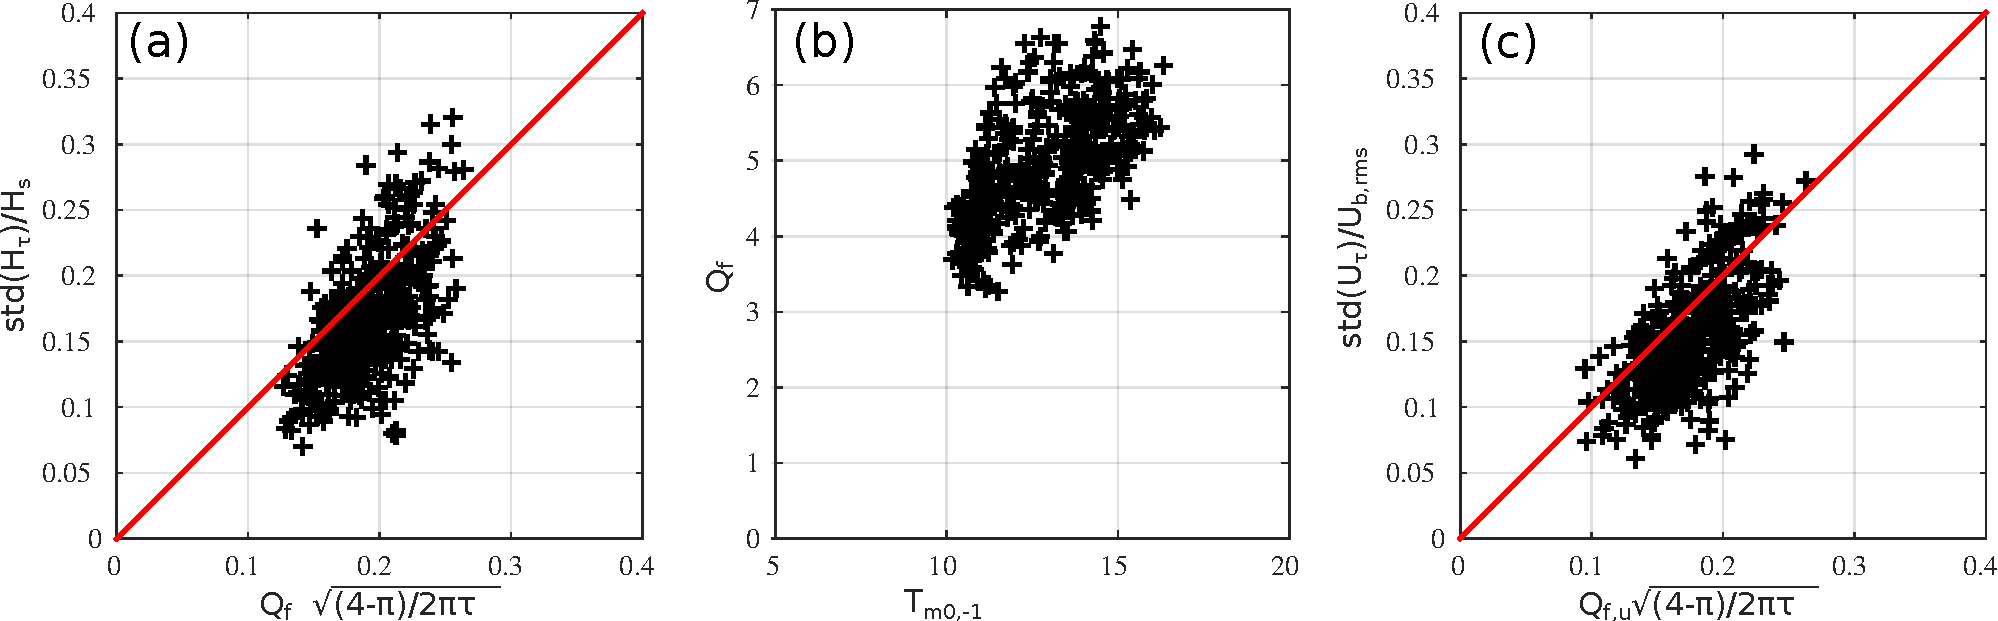
\includegraphics[width=\textwidth]{FIGS_CH_GROUPS/Qf_test.pdf}}
%\vspace{3.64in}
  \caption{Variability of measured parameters over 21 days of measurements in Bertheaume bay, January 2004 using $\tau=180$~s and each symbol corresponds to 1 hour of data: (a) Standard deviation of $H_{\tau}$ normalized by $H_s$ as a function  of the predicted variability using $Q_f$ (b) correlation of $Q_f$ and the mean period $T_{m0,-1}$, (c) variability of bottom orbital velocity amplitude $U_{b,\mathrm{rms}}$ against the relevant $Q_{f,u}$ peakedness parameter.}
\label{fig:groupsQf}
\end{figure}
%%%%%%%%%%%%%%%%%%%%%%%%%%%%%%%%%%%%%%%%%%%%%%%%%%%%%%%
Figure \ref{fig:groupsQf}.a shows that the predicted variability is not exactly like the estimated variability, but it provides a useful order of magnitude, with the "noise" on wave height estimate decreasing like $\sqrt{1/\tau}$, which is why wave records are normally taken over 20 minutes. In the present case, using $2\tau = 20$ minutes averaging instead of averaging over $2\tau = 3$~minutes reduces statistical uncertainties by a factor $\sqrt{20/3}=2.6$, giving a mean value of $\mathrm{std}(H_\tau)/ H_s=6.4\%$, which is of the same order of magnitude as the 5\% relative uncertainty for buoy data for wave heights around 2~m  that is estimated from triple-collocation techniques \citep{Dodet&al.2022}. This suggests that sampling errors caused by wave groups are a large part of the uncertainty in buoy data.

It is always possible to average over longer times but at some point one loses the time resolution that may be needed to investigate how the wave height varies during the tidal cycle or due to other fast evolving phenomena. We also note that quantities that involve higher frequency moments of order $n$ such as the orbital velocity with $n=2$ are less "groupy", their spectrum shape given by $E(f)f^n$ are broader than $E(f)$,  and we can compute a similar $Q_f$ for these parameters that will be lower, as shown in  \ref{fig:groupsQf}.c, using the bottom orbital velocity data from the Nortek Vector instrument. I used pressure and velocity at the ocean bottom in Figure \ref{fig:groupsQf}.a and \ref{fig:groupsQf}.c, and these are already filtered by the water depth, so that the difference between these  $Q_f$  and  $Q_{f,u}$ is not as large as it would be if one used surface elevation and surface velocity.  


\subsection{Spatial maps}
Following the same steps we took for time series, we may imagine that an instrument provides a wave height  $H_{L}$ from a spatial average over a 
square of side $L$ \citep{Lenain&al.2024,Ardhuin&al.2024}. The wave height estimate $H_L$ is  again a $\chi$-distributed random variable with its variance and mean given by  functions of the number of 
degrees of freedom, and their ratio given by eq. (\ref{eq:groups_var_nu}). The only difference is that now  $\nu_{f,H}$ is replaced by 
\begin{equation} 
\nu_{\mathrm{kk},H}=1/ Q_{\mathrm{kk},H}^2 dk_x dk_y \label{eq:nukk}
\end{equation}

 where $dk_x dk_y$ is the spectral resolution of the spectral analysis, corresponding to $dk_x dk_y=(2 \pi)^2/(2 L)^2$, with 
\begin{equation} 
   Q_{\mathrm{kk}}^2 = \frac{  \int_{-\infty}^\infty \int_{-\infty}^\infty E^2(k_x,k_y)\mathrm{d}k_x \mathrm{d}k_y }{\left( \int_{-\infty}^\infty \int_{-\infty}^\infty E(k_x,k_y)\mathrm{d}k_x \mathrm{d}k_y  \right)^2} \label{eq:Qkk},
\end{equation}
where  $E(k_x,k_y)$ is the centrally symmetric double-sided spectrum. If one uses the single-sided spectrum instead, as we did for frequency spectra in eq. (\ref{eq:Qf}), the numerator of eq. (\ref{eq:nukk}) should be 2, as in  eq. (\ref{eq:nuf}). 

This expression is easily verified by taking a wave spectrum $E(k_x,k_y)$, simulating the ocean surface map $\zeta(x,y)$ using random phases, and computing the variance over square tiles of side $L$, as illustrated in Fig. \ref{fig:groups_maps}. The theory, combining eq. (\ref{eq:nukk}) and eq. (\ref{eq:groups_var_nu}) gives 
\begin{equation} 
 \frac{\mathrm{std}(H_L)}{\mathrm{mean}(H_L)} \simeq \pi \sqrt{2}  Q_{\mathrm{kk}} /  L,
   \label{eq:groups_var_2DY}
\end{equation}
which a good approximation in cases where $L$ is much larger than the dominant wavelength. 
%%%%%%%%%%%%%%%%%%%%%%%%%%%%%%%%%%%%%%%%%%%%%%%%%%%%%%%
\begin{figure}[htb]
\centerline{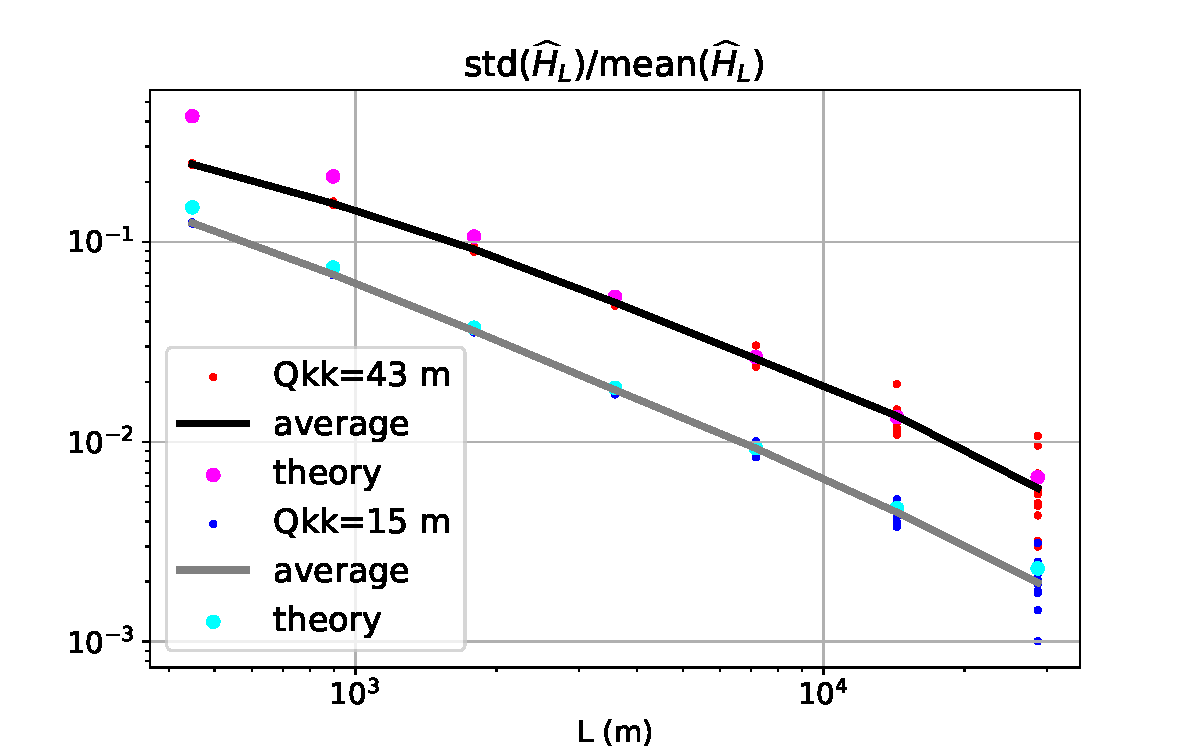
\includegraphics[width=0.8\textwidth]{FIGS_CH_GROUPS/std_maps.pdf}}
%\vspace{3.64in}
  \caption{Variability of $H_L$ in simulated surfaces from 2 different wave spectra, one with $Q_{\mathrm{kk}}=43$~m and the other with $Q_{\mathrm{kk}}=15$~m. These two spectra are shown below in Fig. \ref{figure:groups_storm2}. for each spectrum, 10 surface realisations were generated using random phases, and the average standard deviation is compared to the 
  theoretical value from eq. (\ref{eq:groups_var_2DY}). The notebook that generated this figure is available on \href{https://github.com/ardhuin/waves_in_geosciences/blob/main/NOTEBOOKS/chapter_groups_figure_Qkk_stdH_2D_maps.ipynb}{github}.}
\label{fig:groups_maps}
\end{figure}
%%%%%%%%%%%%%%%%%%%%%%%%%%%%%%%%%%%%%%%%%%%%%%%%%%%%%%%


\subsection{Along-track variability in altimeter data}
A practical important application of the result above is the interpretation of the most common measurement of wave heights from space: using satellite altimeters. Although the details will be given only in the next chapters, we may guess that an altimeter samples the ocean with some filtering function that not a square boxcar but some sort of disc of radius $r$, and  we can imagine that the local height is some convolution of the envelope
\begin{equation}
    H_{r}(x,y) = 4\sqrt{\frac{2}{\pi}} (\eta \otimes g_{r})(x,y).
   \label{eq:relation_Hs_eta}
\end{equation}
In practice a single altimeter gives estimates along a single track in the $(x,y)$ plane and the filter function $g_r$ can be a little complicated. For Delay-only altimeters the detailed form of $g_r$ was derived in \cite{DeCarlo&al.2023}, and for our purpose a good approximation is a a Gaussian filter of radius $r_a=r_C/4.5$, giving a filter $G_{r_a}=\exp{(-k^2 r_a^2)}$ for the power spectrum in Fourier space with $r_C$ given by \cite{Chelton&al.1989} as the radius of the region of the ocean surface that may contribute to the measured signal (again, details will follow in the next chapter), 
\begin{equation}
    r_C =\sqrt{\frac{ 2 h_o H_s+ 2 \delta_R}{1+h_o/R_E}} \label{eq:rC}
\end{equation}
where $h_o$ is the satellite orbit height above the ocean, $R_E$ is the Earth radius and $\delta_R$ is the range resolution of the altimeter.  
 
 
Using the double-sided wave spectrum $E(k_x,k_y)$ of the surface elevation, defined for $(k_x,k_y)$ in the entire wavenumber plane and centrally symmetric, the region of the envelope spectrum for $k \ll k_p$, with $k_p$ the wavenumber peak, is 
proportional to
\begin{equation}
    \Psi_{2}(k_x,k_y) = 8 \int_{-\infty}^\infty 
    \int_{-\infty}^\infty
E(u,v)E(u+k_x,v+k_y)\mathrm{d}u \mathrm{d}v,
\end{equation}
in which $\Psi_{2}$ is also double-sided. From  eq.~(\ref{eq:relation_Hs_eta}), the spectrum of $H_r$ is
\begin{eqnarray}
\Psi_{H_r}(k_x,k_y) &= & \frac{32}{\pi}  \Psi(k)  G_{r}(k_x,k_y) =  \underbrace{\frac{32}{\pi} \frac{8 - 2\pi}{H_s^2}   \Psi_2(k_x,k_y)}_{\Psi_{H_0}(k_x,k_y)}  G_{r}(k_x,k_y)\label{eq:eq2_inFourier}
\end{eqnarray}
with $H_s$ the usual significant wave height and $G_{r}=G_{r_a}$ when considering a single altimeter measurement.

We will now average data along the track, which is the usual practice, at least over 0.05~s corresponding to the 20~Hz rawest data downlinked for most instruments, and corresponding to 350~m distance along the track. For delay-only measurements, these data are fairly noisy and most users typically use at least 1~Hz data (averaged over 7~km) or longer time averages. For simplicity we take the satellite track along the $x$-axis, and we consider an averaging length $d_1$. 
Integrating $\Psi$ for $k_x > k_1$, amounts to integrating $\Psi_{H_r}(k_x,k_y)$ to get the expected variance up to the  cut-off wavenumber along $k_x$, $k_1\simeq \pi / d_1 $, giving $\mathrm{var}(H_{r},d_1)$, the group-induced fluctuations of $\widehat{H}_s$ 
\begin{equation}
\mathrm{var}(H_{r}, d_1) = \int_{-\infty}^{\infty} \int_{k_x > |k_1| } \Psi_{H_0}(k_x,k_y)  G_{r}(k_x,k_y) \mathrm{d}k_x \mathrm{d}k_y. \label{eq:varfromspec2D}
\end{equation}
% pi/2 * (2/ra^2 - 4 k1 / sqrt(pi) ra) = pi * ka^2 - 2 ka*2k1  ka = 
Here again, if the filter $G_{r}$ is zero outside of a very small range of wavenumbers, we can approximate $\Psi_{H_0}(k_x,k_y) \simeq \Psi_{H_0}(k_x=0,k_y=0)$ and take this value out of the integral, and the integral is related to the effective area of the filter in the wavenumber plane which we approximate as a disk of radius $1/r_a$, with an area $\pi /r_a^2$, given by the integral of $G_{r}$ over the entire wavenumber plane, and we remove a band of width $2 k_1$ and length $2/r_a$ because we are only averaging over $d_1$ so that wavelengths longer than $2 d_1$ cannot contribute to our signal and must be excluded. This gives,  
\begin{eqnarray}
    \mathrm{var}(H_{r},d_1) &\simeq&  \Psi_{H_0}(0,0)   \int_{-\infty}^{\infty} \int_{k_x > |k_1| } G_{r}(k_x,k_y) \mathrm{d}k_x \mathrm{d}k_y \nonumber \\
    &\simeq&  \Psi_{H_0}(0,0)  \pi\left(1 / {r_a}^2 - 4 k_1/ r_a \right) \nonumber\\
    &\simeq&  \frac{32}{\pi} \frac{8 - 2\pi}{H_s^2}   \Psi_2(0,0)   \pi  \left(1 / {r_a}^2 - 4 k_1/ r_a \right) \nonumber\\
    &\simeq&   Q_{kk}^2 H_s^2(8 - 2 \pi) \left(1 / {r_a}^2 - 4 k_1/ r_a \right)  , 
\end{eqnarray}
where we have defined 
a two-dimensional spectral peakedness $Q_{kk}$ which is measured in meters,
\begin{equation}
    Q_{kk}^2 = \frac{\iint_{} E^2(k_x,k_y)\mathrm{d}k_x\mathrm{d}k_y}{\left(\iint_{}E(k_x,k_y) \mathrm{d}k_x\mathrm{d}k_y\right)^2} = \frac{32 \Psi_2(k_x=0,k_y=0)}{H_s^4}.
\label{eq:bandwith_2D}
\end{equation}


This expression gives the approximate value for the standard deviation,
\begin{equation}
    \mathrm{std}(H_{r},d_1) \simeq  H_s   Q_{kk}  \sqrt{ (4-\pi) \left[2/r_a^2 -  8 k_1 / r_a\right] }.\label{eq:Lambda2}
\end{equation}

{This variability of $H_{r_a}$, which we have defined as the contribution of wave groups to the variability of measured wave heights $\widehat{H}_s$ is thus the product of three factors: the significant wave height $H_s$, the shape of the wave spectrum as quantified by $Q_{kk}$, and the effective range of spatial scales over which the variance is integrated. That last factor is a function of the smoothing effect of the altimeter, represented by the filtering scale $r_a$, and the distance $d_1=2\pi / k_1$ over which  we consider the variability.


%%%%%%%%%%%%%%%%%%%%%%%%%%%%%%%
\begin{figure}[h!]
\centerline{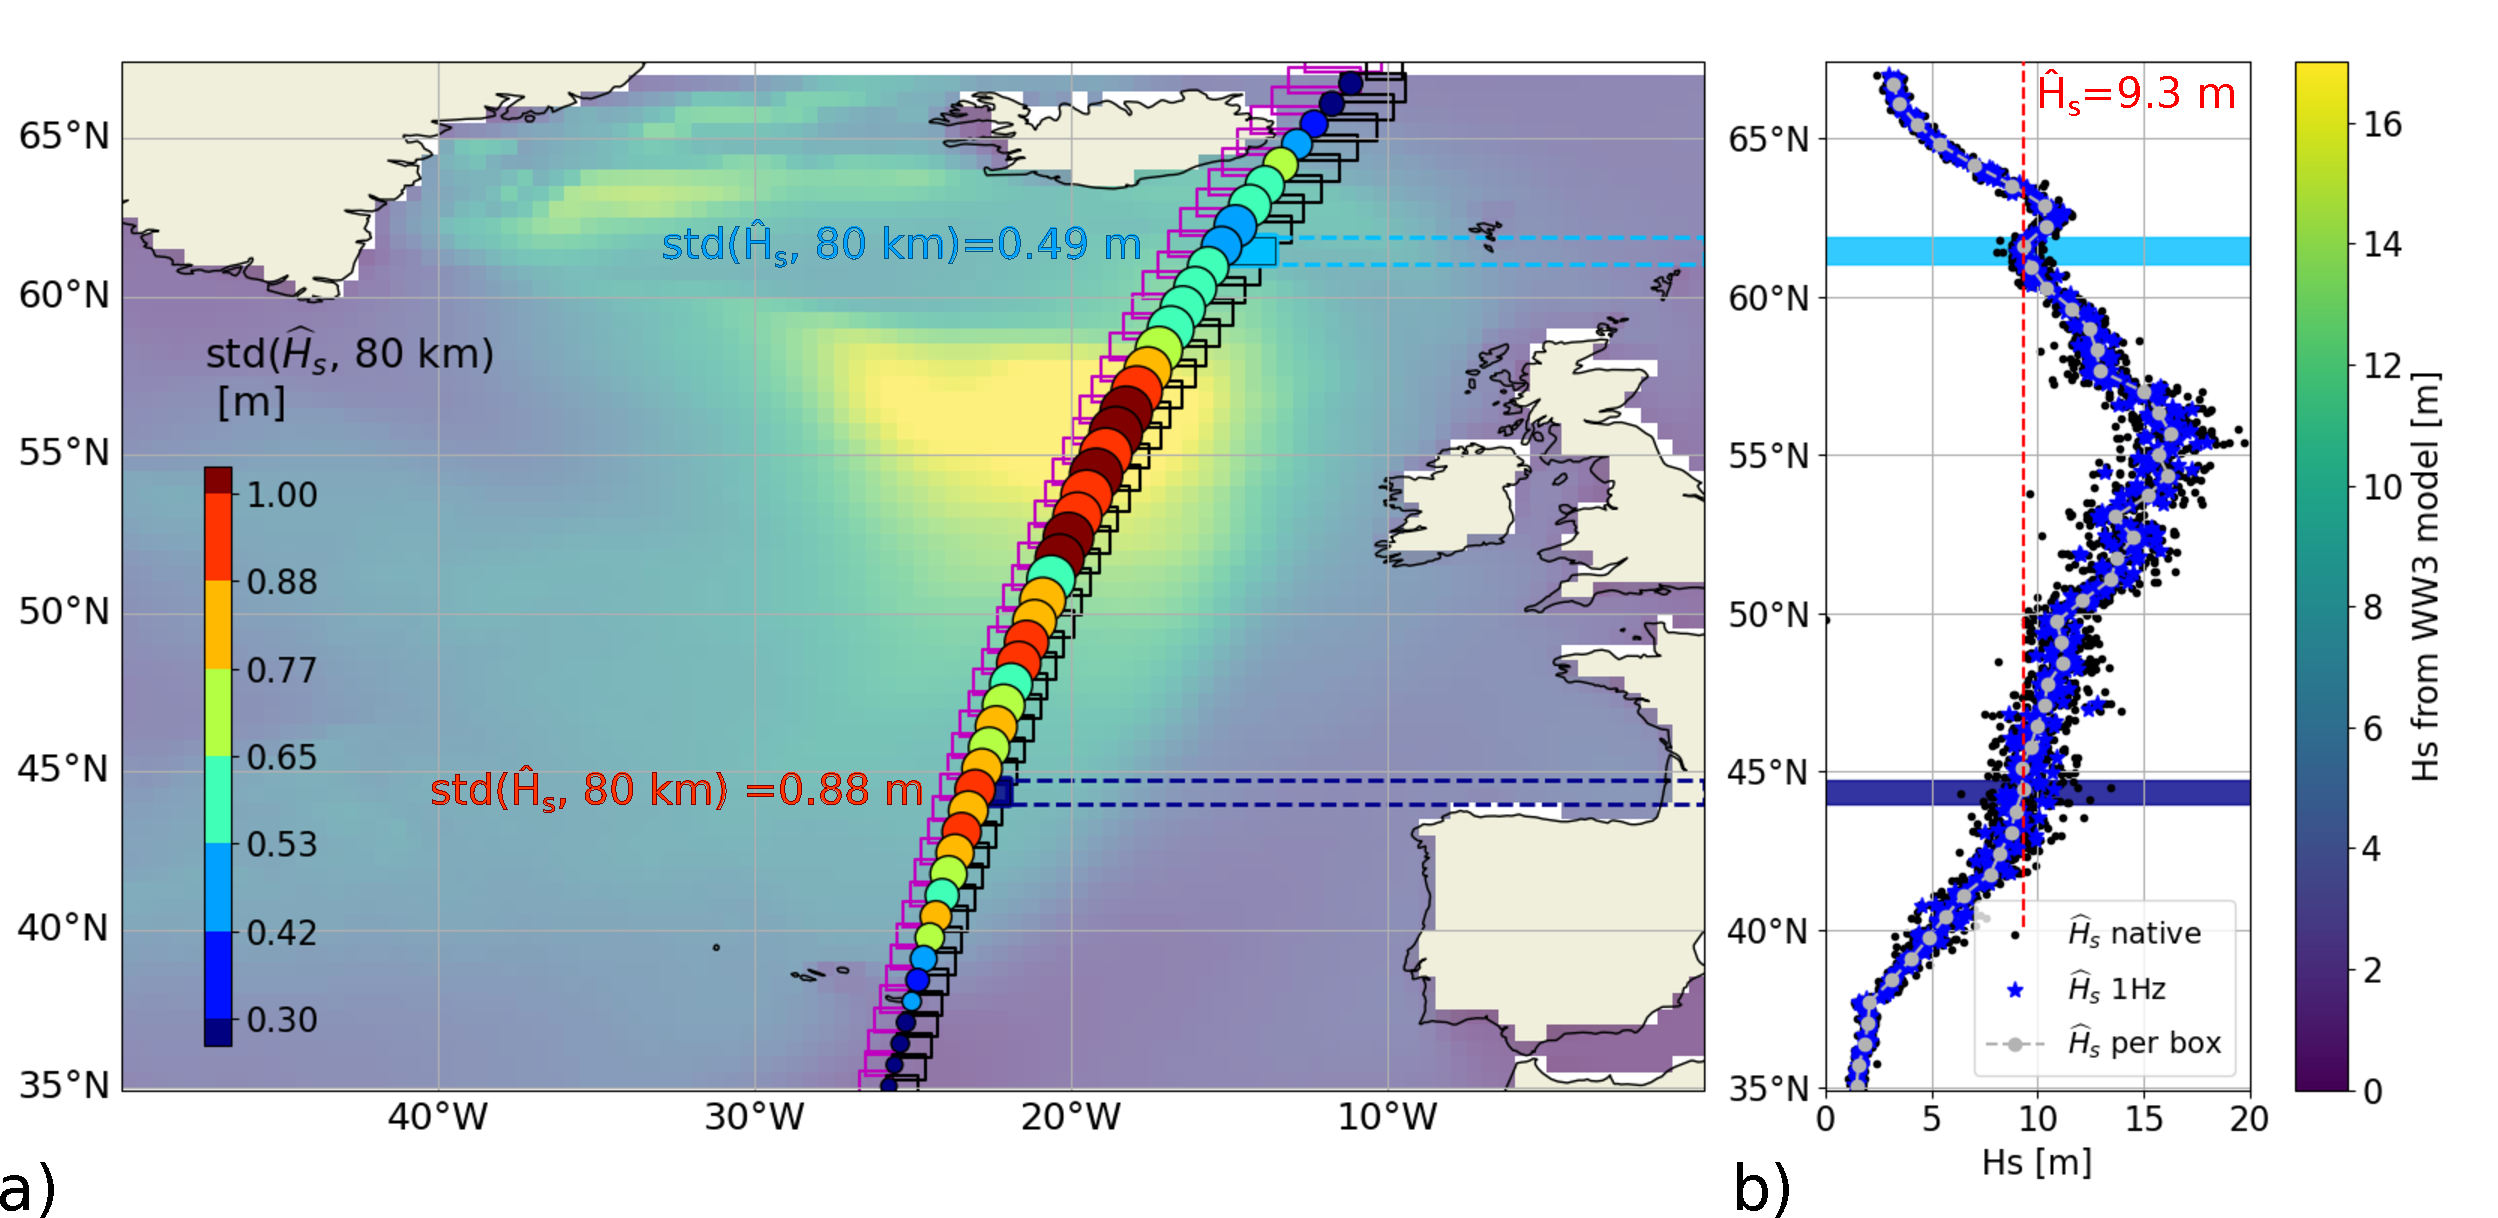
\includegraphics[width=\textwidth]{FIGS_CH_GROUPS/DeCarlo_fig1.pdf}}
    \caption{a) Map of wave heights in the North Atlantic at 09:00 on 14 February 2020, as provided by the model hindcast of \cite{Alday&al.2021}, overlaid with circles located at the center of SWIM box estimates for the L2-CWWIC wave spectra. Circles are sized by the L2-CWWIC $H_s$ estimate and color corresponds to $\mathrm{std}(Hs)$; b) corresponding measured $H_s$ values as a function of latitude (y-axis) : black small dots represent native measurements at 4.5 Hz, blue stars represent the 1~Hz averaged and grey circles represent the $H_s$ averaged over a box. Two boxes are selected for the case study: box A - highlighted in light blue - is at 62$^\circ$N, and box B - in dark blue - is at 44$^\circ$N.} 
   \label{figure:groups_storm1}
\end{figure}
%%%%%%%%%%%%%%%%%%%%%%%%%%%%%%%
This work on the variability of wave height estimates was started after finding a much larger variability on the south side of storm Dennis in the North Atlantic in 2020, as illustrated in Fig. \ref{figure:groups_storm1}. We used CFOSAT because the SWIM instrument has a nadir (vertical) beam working like an altimeter, and slanted beams that give a measure of the directional spectrum which we can use to compute $\Psi$, the spectrum of the envelope. The maximum value of $H_s$ reported by CFOSAT in the storm was estimated at 17.9~m when using a the average over one measurement cycle (there are 4.5 such measurements per second), or 17.9~m when averaged over 1 s. More interesting to us was, for the same mean wave height of 9.3~m, a very small variability on the north side, and a twice larger variability on the south side. 

Taking the measured wave spectra and simulating the surface and its envelope, as done in Fig. \ref{figure:groups_storm2} makes it easier to visualize the importance of the spectral shape for the defining the spatial variability of wave heights $H_r$. Both panels (c) and (d) correspond to spatially homogeneous sea states with a uniform $H_s$. However, any measurement of waves will be sensitive to the "lumps" of high values and low values that are best seen in the envelope map of Fig. \ref{figure:groups_storm2}.f. The only way to remove this effect of wave groups in the measurements would be to average in time as these groups propagate fast and randomly appear and disappear. 

%%%%%%%%%%%%%%%%%%%%%%%%%%%%%%%
\begin{figure}[hbt!]
\centerline{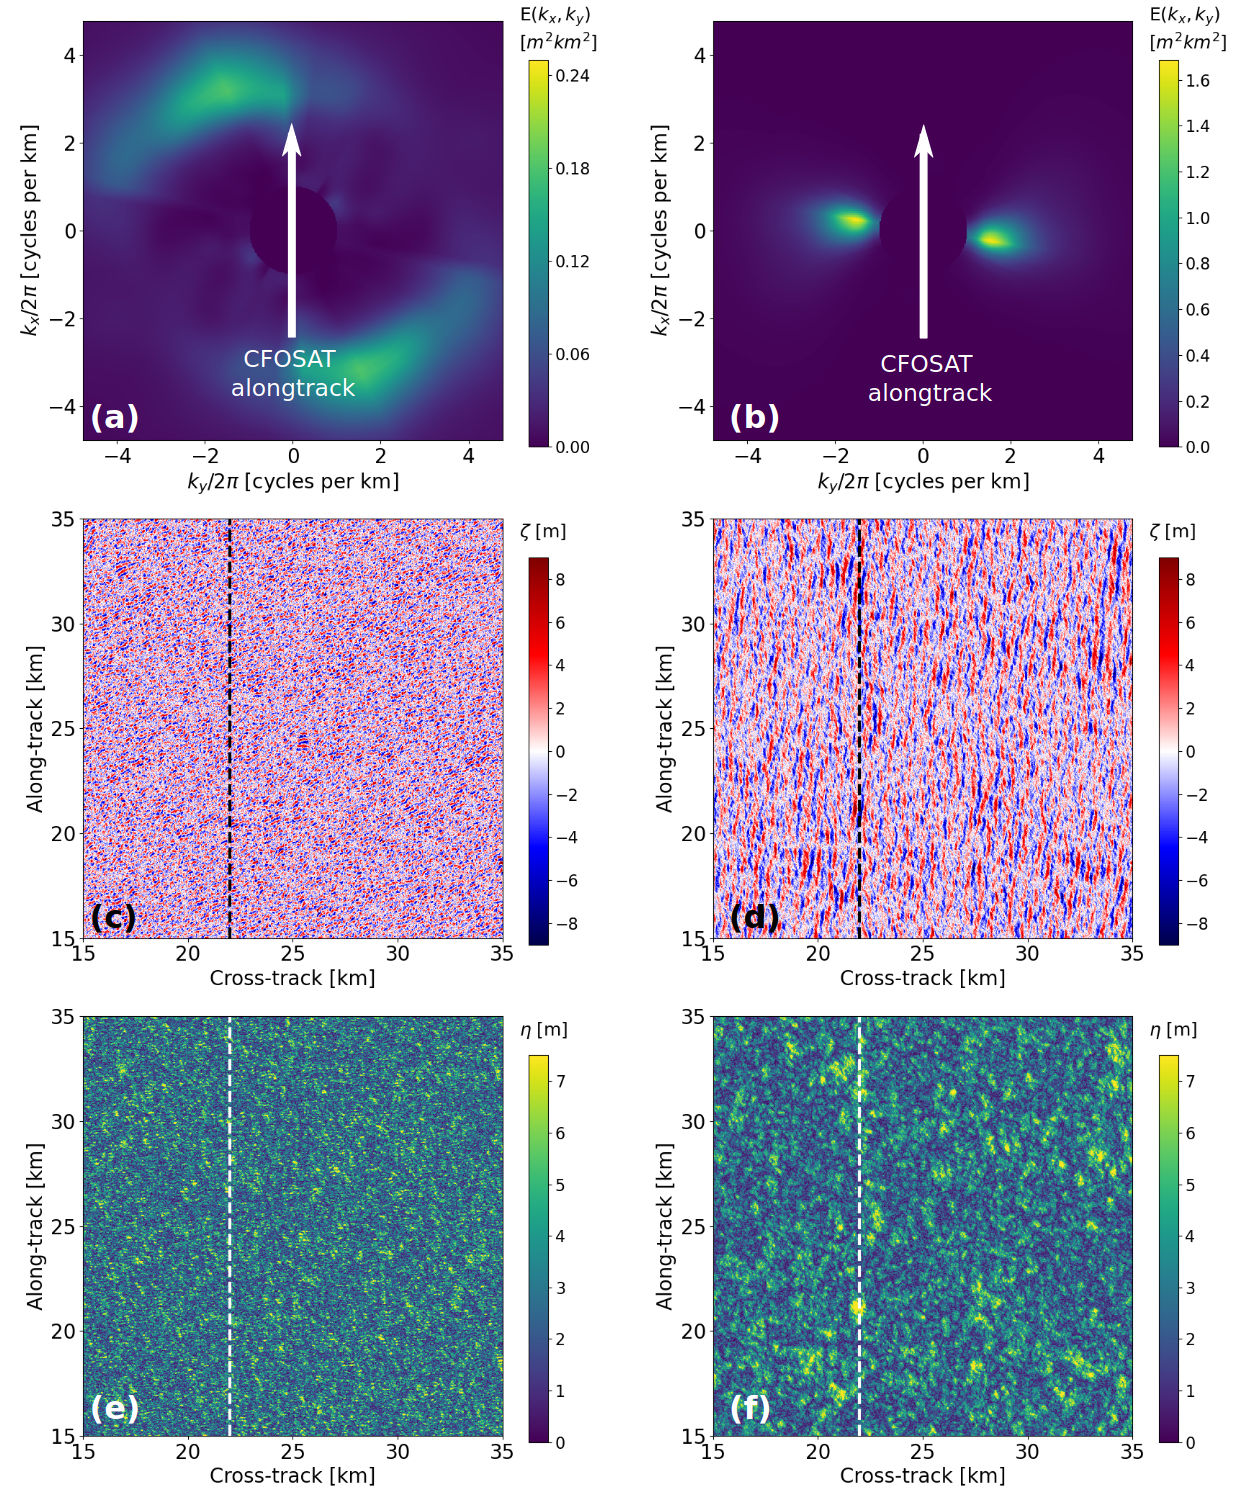
\includegraphics[width=0.8\textwidth]{FIGS_CH_GROUPS/DeCarlo_fig2.jpg}}
    \caption{From wave spectra (top) to surface elevation envelope (bottom): the surface elevations maps in the middle line are simulated using the CFOSAT-derived spectra (these are L2S product corrected to give the same wave height as the nadir beam), with random phases. Combining the real and imaginary parts of the simulated surface gives the envelope. The left column is for a broad wave spectrum with a lower peak period. The right column has the same wave height but a long peak period and narrower spectrum. } 
   \label{figure:groups_storm2}
\end{figure}
%%%%%%%%%%%%%%%%%%%%%%%%%%%%%%%

We can use our theory to verify that in the case of narrow spectra, the expected effect of wave groups gives a standard deviatin of the estimates of wave heights $H_r$ that is similar to the standard deviation of the measurement over a 80~km segment along the satellite track (Fig. \ref{figure:groups_storm3}). 
%%%%%%%%%%%%%%%%%%%%%%%%%%%%%%%
\begin{figure}[ht!]
\centerline{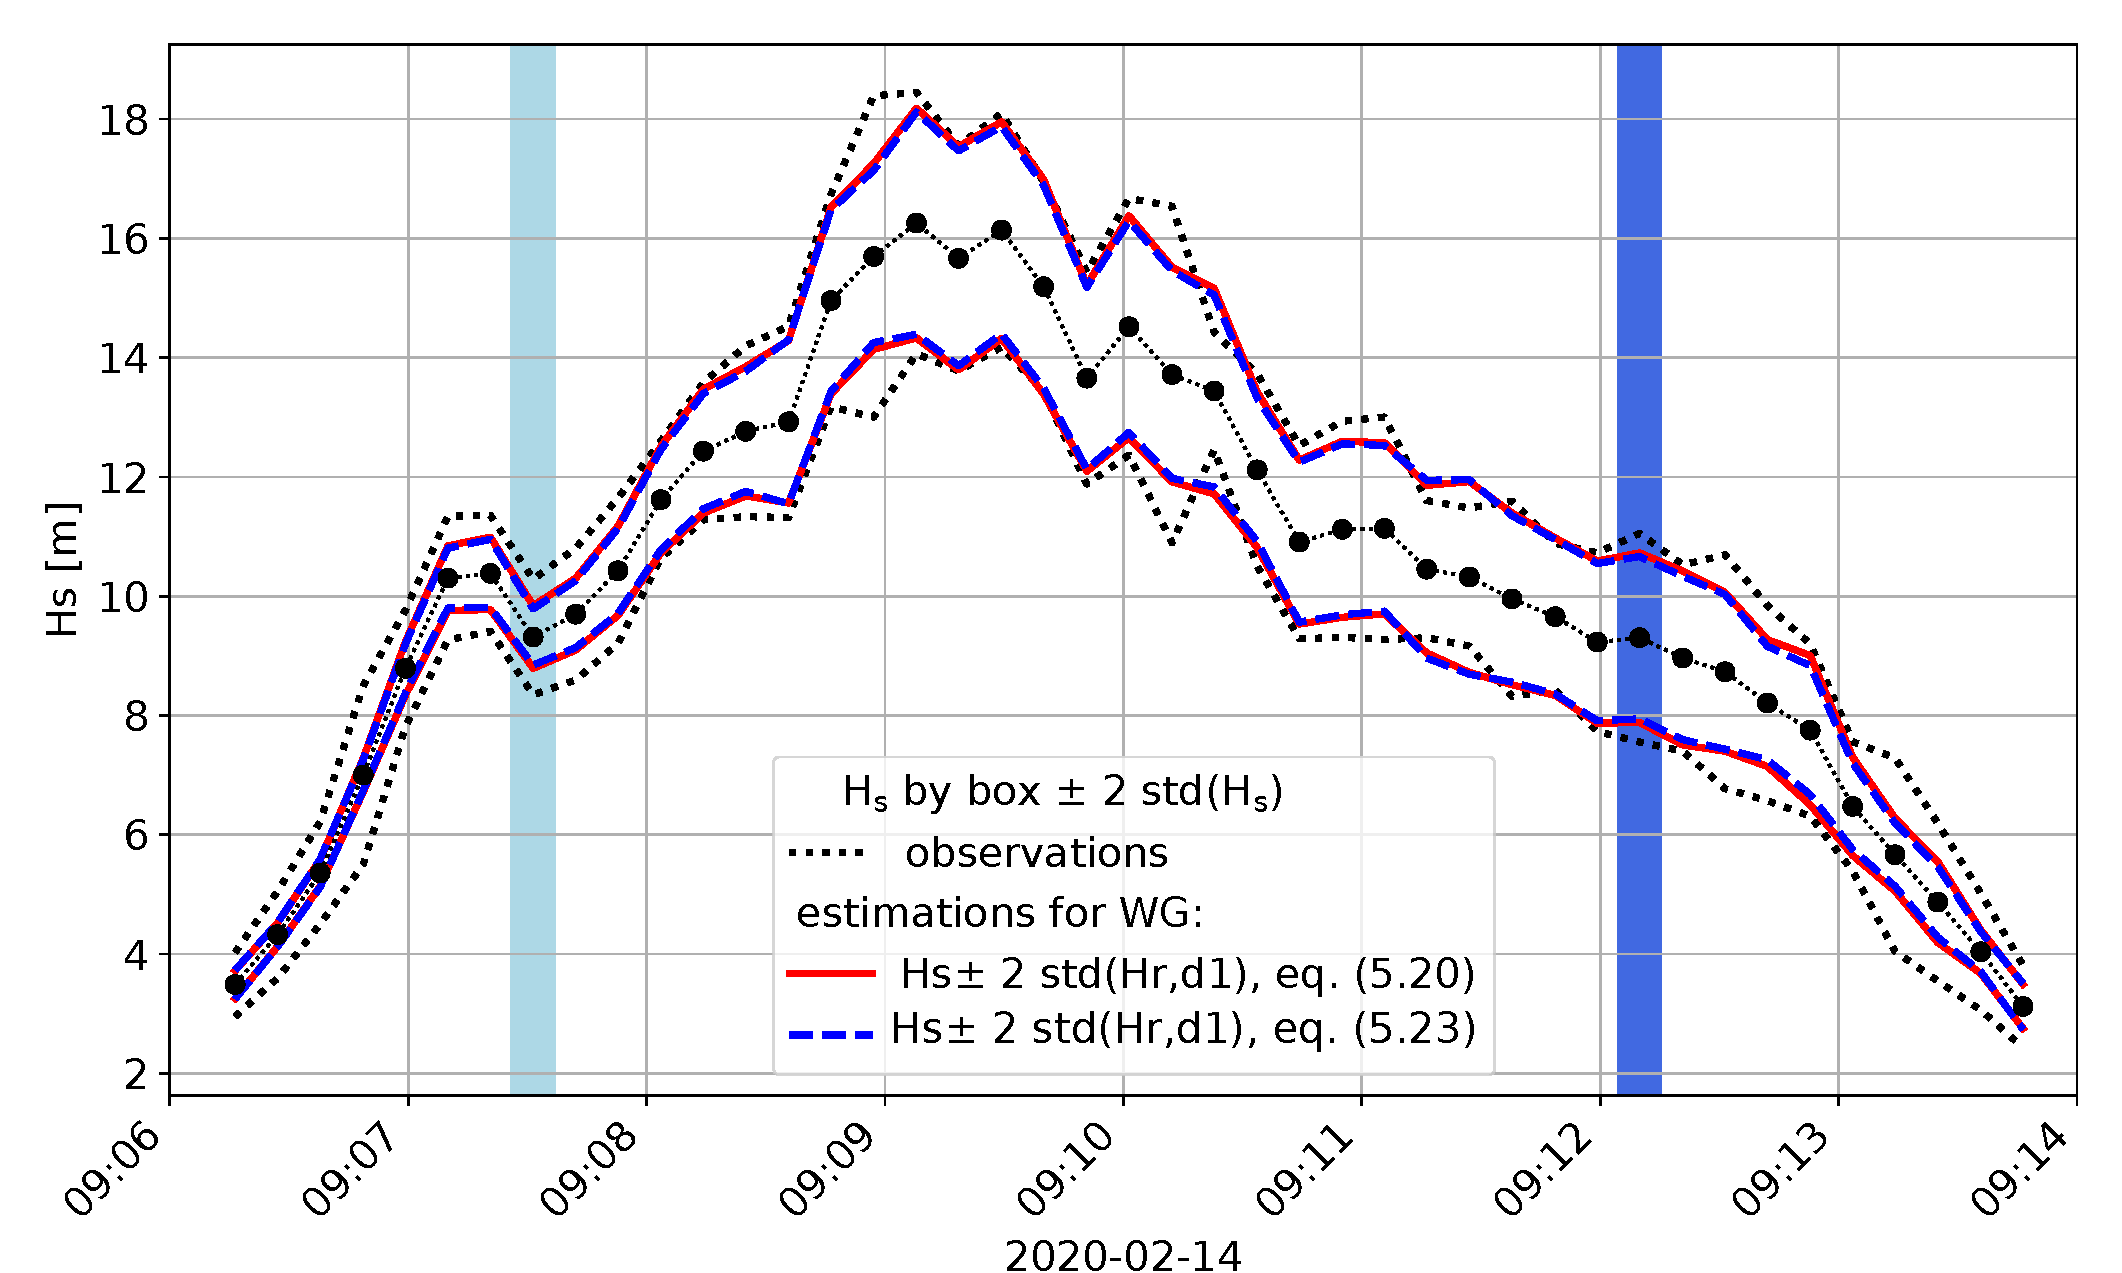
\includegraphics[width=0.75\textwidth]{FIGS_CH_GROUPS/groups_Storm_Dennis_2023_fig3.pdf}}
    \caption{Values of measured $H_s$, averaged over 80~km - black circles - ,  and corresponding $\mathrm{std}(Hs)$ - black dash-dotted lines - in the satellite data, for the CFOSAT track shown in Fig.~\ref{figure:groups_storm1}. Estimations of $\mathrm{std}(H_r,d_1)$ are also represented - in red and blue.} 
   \label{figure:groups_storm3}
\end{figure}
%%%%%%%%%%%%%%%%%%%%%%%%%%%%%%%
On the contrary, for the broader wave spectrum, the effect of wave groups is much smaller than in the measurements: it is possible that the data contains true gradients of the underlying $H_s$, and we also know that measurement noise (known as speckle) is often the dominant source of variability in the measured values. This is one of the main reason for the development of Delay-Doppler altimetry which has a much lower level of speckle noise due to the averaging of different indepedent Doppler "looks" for the same measurement. 

In their paper \cite{DeCarlo&al.2023} went on to show that one can remove the predicted "group-induced noise" in the wave height measurements to produce maps of wave height "noise" that now clearly show that small scale variability in wave heights is clearly associated with regions of strong mesoscale currents, as we will see in chapter \ref{ch_current}.

